\documentclass[11pt]{article}
\usepackage{royden-report}
\usepackage[T1]{fontenc}
\usepackage{lmodern,microtype,array,longtable,enumitem}
\setlist{itemsep=3pt,topsep=5pt}
\newcommand{\D}{\lvert D_\tau\rvert}
\newcommand{\TT}{\mathbb T_L}
\newcommand{\norm}[1]{\lVert #1\rVert}
\newcommand{\abs}[1]{\lvert #1\rvert}
\newcommand{\dd}{\,\mathrm d}
\newcommand{\F}{\mathcal F}
\newcommand{\testgoal}[1]{\paragraph{Goal.}#1}
\newcommand{\testdesign}[1]{\paragraph{Experiment and control.}#1}
\newcommand{\testdecision}[1]{\paragraph{Decision and limitation.}#1}
\title{Learning Dysthe Evolution Across Initial Wave Fields\\
\large A literature-grounded numerical, FNO, and PINN research protocol}
\author{}
\date{25 October 2026}
\hypersetup{pdftitle={Learning Dysthe Evolution Across Initial Wave Fields},
pdfsubject={Spatial water-wave Dysthe: numerical qualification, operator learning, and long-distance evaluation}}
\begin{document}
\maketitle
\begin{abstract}
The proposed goal is to learn the evolution of a bounded family of complex
water-wave envelopes and establish how far predictions remain accurate on
unseen initial fields. Begin with the approved spatial free-surface Dysthe
equation, a qualified Fourier reference, and a short-distance Fourier neural
operator (FNO). Compare the same architecture with and without a full
equation residual; use an ordinary physics-informed neural network (PINN)
on a small set of individual problems to diagnose physics training.
A function-conditioned PINN is an optional operator comparison.
Success means accurate modulation growth, focusing, recurrence and spectral
transfer at a measured cost and within a declared validity range.
It does not mean all-distance accuracy or a proof of global smoothness.
This report reviews primary literature, audits the current implementation,
specifies data and acceptance gates, and supplies small independent
operator checks. No FNO/PINN was trained and no new long-distance evolution
campaign was run for this review.
\end{abstract}

\section{The question and the proposed contribution}
\label{sec:goal}

\begin{quote}
For a specified family of smooth initial free-surface envelopes, can a
learned solution operator predict unseen wave fields and their modulation
events over longer propagation distances, with controlled error and useful
amortized cost relative to a tuned numerical solver?
\end{quote}

This question has three separately measurable parts. First, learn a map
across initial fields, rather than fitting a single trajectory. Second,
determine the distance over which repeated predictions remain qualified.
Third, test whether the method retains the particular water-wave effects
for which Dysthe corrections are useful. Reproducing known modulation
phenomena is validation; a reproducible improvement in generalization,
accuracy per unit cost, or reliable prediction distance would be the
methodological contribution. Novel wave physics is not assumed.

The first comparison should be a supervised FNO and the same
distance-conditioned FNO with a physics loss, commonly called a
physics-informed neural operator (PINO). The FNO and PINO literature
supports these method classes, but does not establish their performance
on this Dysthe problem \cite{fno,pino}. An ordinary PINN trained for each
initial field answers a different question and incurs new optimization
cost for every field. A branch-conditioned physics-informed operator
can answer the multi-input question \cite{deeponet,pideeponet}.

Water-wave studies provide closer precedents. Ehlers et al. fit a
separate complex-output NLS PINN to synthetic sparse-gauge data, with
coefficient identification for model mismatch; Dysthe appears as future
work \cite{ehlers2024}. Ehlers, Stender and Hoffmann use an FNO-based
PINO with high-order-spectral free-surface residuals to reconstruct
phase-resolved surfaces across sensor inputs \cite{ehlers2025}.
Eeltink et al. combine viscous MNLS with LSTM corrections learned from
breaking-wave experiments; their magnitude and spectral-magnitude
targets and wave-type-dependent corrections do not validate complex
inviscid rollouts \cite{eeltink}. These precedents motivate distinguishing
instance fitting from operator generalization, fixed-equation
approximation from missing-physics correction, and reconstruction from
autonomous propagation. This is a focused methods review, not a claim
of first use or an exhaustive priority search.

Three proposed hypotheses make negative results useful:
\begin{enumerate}
\item A short-distance FNO generalizes within a bounded initial-data
distribution at a declared error tolerance.
\item Adding a correctly evaluated residual improves held-out rollout
accuracy or reduces the amount of reference data required, after
accounting for its extra cost.
\item Short rollout training extends the reliable prediction distance
without suppressing true modulational instability.
\end{enumerate}
Failure of any hypothesis is a legitimate result. None implies a
statement about existence of the underlying PDE.

\begin{figure}[htbp]
\centering
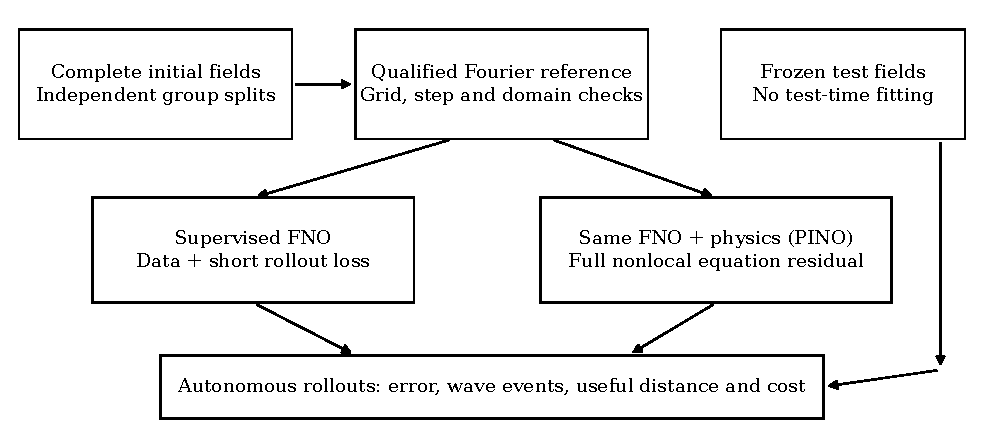
\includegraphics[width=\linewidth]{comparison_design.pdf}
\caption{The first controlled comparison. Both models share a representation
and data population; only the physics term differs. The ordinary per-input
PINN is a separate, smaller diagnostic experiment. This is an experimental
design, not a plot of completed results.}
\label{fig:comparison}
\end{figure}

\section{Fix the equation before comparing methods}
\label{sec:model}
On the periodic profile interval $\TT=\RR/L\ZZ$, the approved
\texttt{water-wave-dysthe-spatial-v1} initial-value problem is
\begin{align}
\partial_\xi u=F_\epsilon(u)
&=-i u_{\tau\tau}-i|u|^2u \notag\\
&\quad-\epsilon\left(8|u|^2u_\tau
+2u^2\overline{u_\tau}+2iu\D(|u|^2)\right),
\qquad u(0,\tau)=u_0(\tau).
\label{eq:baseline}
\end{align}
Here $\xi$ is propagation distance and $\tau$ is retarded profile time.
This is the free-surface equation with coefficients
$(a,h,c,e,f)=(1,1,8,2,2)$ in Fedele--Dutykh's displayed equation (1.3)
\cite{fedele}. In particular the conjugate derivative term is present.
A velocity-potential envelope has different coefficients.

For $k_m=2\pi m/L$, use
\[
\widehat f_m=\frac1L\int_{\TT}f(\tau)e^{-ik_m\tau}\dd\tau,\qquad
\widehat{\D f}_m=|k_m|\widehat f_m,\qquad \widehat{\D f}_0=0.
\]
Thus the Hilbert-transform multiplier is $-i\,\mathrm{sign}(k)$ and
$\mathcal H\partial_\tau=\D$. The linear propagator has multiplier
$e^{ik_m^2s}$, not $e^{-ik_m^2s}$.
The stated carrier normalization is
$\tau=\epsilon(2x-t)$, $\xi=\epsilon^2x$, and $B=\epsilon u$.
The $\epsilon=0$ equation is a mathematical NLS control; that change of
physical coordinates cannot be inverted at zero.

When a sufficiently regular solution exists on $[0,s]$, write its map as
$\mathcal S_s^\epsilon:u_0\mapsto u(s,\cdot)$. This notation presupposes a
well-defined solution on that interval. An operator-approximation theorem
does not construct that solution or prove its global existence.

\subsection{How the two supplied papers enter this project}
Dysthe's 1979 paper derives a temporal potential-envelope correction and
studies sideband instability \cite{dysthe1979}. It motivates the mean-flow
term and a modulation-growth test. Its variables, dimensionality and
coefficients cannot be pasted into \eqref{eq:baseline}.
The supplied Schober--Islas preprint develops a weakly viscous hierarchy
and a separate finite-adjustment-time mean-flow closure
\cite{schober}. It motivates a future, separately specified dissipative
study. It neither supplies an operator-learning algorithm nor proves
continued smoothness for the present spatial equation.

The earlier companion review, \emph{Dysthe Evolution: Numerical Evidence
and Existence} (23 October 2026), records two apparent linear-dispersion
inconsistencies in the supplied version 1 and distinguishes its real
relaxation closure from a complex damping coefficient. Those issues
must be resolved before implementing that extension. The present plan
keeps the inviscid spatial model fixed; it does not silently introduce
viscosity, transverse coordinates, or a different envelope variable.

\subsection{What currently exists}
The five active repositories agree on the model and case schema.
The local core supplies complex128 Fourier differentiation, projected
nonlinear products, integrating-factor RK4, and diagnostics. It keeps
$|m|<N/4$, which provides room for its cubic products. The learning
registry still marks all methods unimplemented: there is no active
water-wave FNO/PINN training pipeline.

Stored short runs at $\epsilon=.025$, $L=160$, $N=4096$,
$h=.00125$, $\Xi=4$ include profile, perturbed-profile and Gaussian
qualification records. Their largest stored raw relative $L^2$
grid discrepancy is about $4.2\times10^{-15}$, step discrepancy
$4.1\times10^{-9}$, and domain discrepancy $2.2\times10^{-5}$.
These are historical two-level comparisons for those cases, not
fresh trajectories, error bounds, or evidence for arbitrary inputs.
The Gaussian and solitary archive hashes were freshly checked against
their reports; the core source hash agrees. A historical Gaussian
runner hash differs from today's runner after later formula changes.

A research dataset needs a new bounded generator using the core.
The demonstration runner fixes $\epsilon=.025$, $\Xi\leq4$, and
at most 101 output stations; part of its initializer also hardcodes
that epsilon in provenance. Do not expand the meaning of those records
to cover a new parameter campaign. Before packaging a reproducible run,
align the learning repository's pinned core dependency with the actual
reviewed reference implementation.

\section{Multiple inputs: a declared population, not arbitrary waves}
\label{sec:data}

Begin with $L=160$ and $\epsilon=.025$. A training example contains the
entire complex initial profile, the actual local propagation increment,
and its reference output. Future reference fields are training targets
only. The same trained operator must accept a new initial profile
without optimization. If adaptation is allowed, label and time it
separately.

\subsection{Three complementary input families}
The following ranges are proposed starting values for a bounded pilot,
not ranges established by a physical-validity theorem. Validate a small
batch before freezing them. Record all rejected draws and their reason;
an unreported rejection rule changes the population being learned.

\paragraph{Localized packets: focusing and asymmetry.}
Use a periodized version of
\[
u_0(\tau)=a\exp\left[-\frac{1-ic}{2\sigma^2}(\tau-\tau_0)^2+i\phi\right],
\quad
a\in[.5,1],\quad \sigma\in[6,12],\quad c\in[-.5,.5].
\]
Vary position and phase as well. Periodize the complex function by summing
translated copies, with a documented derivative-level truncation tolerance.
A cropped Gaussian is not exactly periodic. This family tests amplitude,
width, chirp, focusing distance and asymmetric deformation. Hold out
entire parameter draws, not propagation stations. Sech-shaped packets
and two separated packets can later be withheld \emph{families}, not
silently mixed into an interpolation score.

\paragraph{Modulated wavetrains: instability and recurrence.}
Use
\[
u_0(\tau)=a e^{i\phi}
 \left[1+b_+e^{ik_m\tau}+b_-e^{-ik_m\tau}\right].
\]
Choose $a\in[.5,1]$, integer modes spanning stable, near-boundary and
unstable portions of the matrix in Appendix~\ref{app:mi}, and independent
sideband phases. Use $|b_\pm|$ between $.01$ and $.05$ for a nonlinear
pilot; use much smaller paired disturbances for the linearization test.
These waves intentionally fill the periodic domain. They do not need a
localized-packet edge criterion.

\paragraph{Smooth random profiles: functional variation.}
Sample complex Fourier coefficients with a prescribed decaying spectrum,
for example a finite series with $|m|\leq16$ and weights
$\exp[-(m/m_c)^2]$, $m_c\in[4,10]$, followed by a declared RMS-amplitude
choice. Coefficients at $m$ and $-m$ are independent. Bound both peak
amplitude and derivative-weighted bandwidth by rejection or a stated
sampling rule. This is a finite, smooth input distribution with variable
phase, not a claim to represent all sea states. Record its seed and
coefficient vector. An alternative spectral law is a separate
distribution-shift test.

\paragraph{Information that cannot be discarded.}
Intensity $|u_0|^2$ alone does not specify the initial-value problem:
opposite chirps can have the same intensity and different evolution.
Sparse or noisy measurements require an observation model, a
reconstruction method and uncertainty evaluation. They are a later
inverse problem; they must not be presented as another complete-field
input channel with missing phase filled in from the reference.

\subsection{Splits, grids and provenance}
Store reference fields as complex128 arrays $[N_\xi,N_\tau]$ with
$\tau_j=-L/2+jL/N$, excluding the duplicated endpoint. Store explicit
propagation coordinates. The existing runner's rounded output indices
can create unequal increments; validate the actual spacing or condition
the operator on each actual increment.

Assign one immutable \emph{split group} to each base initial draw.
All its windows, refinements, translated or phase-rotated copies,
paired disturbances, and coefficient variants remain in the same split.
Test for duplicate field hashes as well as mislabeled groups.
Generate parameter ranges and seed lists before fitting. Fit global
normalization on training fields only. Use validation for model selection;
open the final test set once the protocol and checkpoint are frozen.
Snapshots from one field are correlated samples, not independent cases.

The current metadata validator is insufficient by itself. The new loader
must check actual shapes, dtypes, finite values, coordinates, hashes,
model ID, epsilon, grid origin, and qualification status. Preserve case
schema 2 and add a separate dataset manifest for group and split records.

Downsample through Fourier restriction, not viewer decimation. Measure
projection and reconstruction errors in $L^2,H^1,H^2,H^3$ over the
qualified reference interval. A 512- or 1024-point learning grid is only a
candidate; require its representation error to consume at most one tenth
of the intended surrogate error budget. Choose the number of learned
Fourier modes through a small validation sweep, such as $32,64,128$,
after inspecting the physical spectra. These numbers do not specify the
FNO output bandwidth.

\subsection{A campaign that can stop early}
Use equal numbers from the three families initially.
\begin{center}
\small
\begin{tabular}{p{.28\linewidth}rrp{.25\linewidth}}
\toprule
Stage & Groups & Train/val/test & Purpose\\
\midrule
Execution smoke & 12 & $6/3/3$ & Load, train, resume and evaluate\\
Bounded pilot & 48 & $36/6/6$ & Select viable method and tolerances\\
Main comparison, if justified & 384 & $288/48/48$ & Estimate held-out performance\\
\bottomrule
\end{tabular}
\end{center}
These are proposed budgets, not power calculations or guaranteed
sufficient sample sizes. Six pilot test groups cannot substantiate broad
generalization. Use learning curves on nested training subsets to decide
whether more groups are useful. Keep the test population fixed while
increasing training data.

At $N=4096$ and 81 saved stations on $[0,4]$, one complex128 trajectory
requires about $5.06$ MiB before compression. Thus 48 and 384 base
trajectories require about 243 MiB and 1.90 GiB, respectively, excluding
refinements and checkpoints. A saved interval $.05$ is a proposed
\emph{learning} increment; the reference integration step $.00125$
is a separate quantity. Extra stations are needed for continuous-distance
training and near fast events.

Qualify representative extremes first, then screen every generated
trajectory; refine any case whose derivative tails or defects approach
the gate. Use full three-level grid and step comparisons on the sentinel
panel and difficult cases, and at least an independent refined
comparison for accepted evaluation cases. Do not assume the three old
demonstrations qualify a whole new distribution.

For the main campaign's first long-distance evaluation, preselect 12 held-out groups
(four per family) by input parameters alone. Extend $4\to8\to16$ and
only then, if useful and qualified, to 32. At 641 stations a 12-case
$N=4096$ panel needs about 481 MiB of base fields. The same panel supports
paired comparisons across methods; do not repeatedly select its easiest
members. Benchmark actual generation and training costs before launching
the main campaign.

Vary epsilon only after the fixed-parameter question works. A proposed
second stage uses $.015,.025,.04$ in training and disjoint groups at
$.02,.03$ for interpolation. Keep $.05$ a separately labeled
extrapolation probe, subject to new qualification and physical screens.
Treat $\epsilon=0$ as an analytic/numerical control. Changing $L$ is a
different domain, and changing transverse dimensionality or dissipation
is a different model.

\section{Implementations that answer the comparison}
\label{sec:learning}

The first comparison should change the training objective while keeping
the representation fixed.  Use $\epsilon=.025$ and $L=160$, and let
$F_\epsilon$ denote the right-hand side of \eqref{eq:baseline}.
An ordinary PINN approximates one solution after its initial condition
has been fixed.  An operator accepts an initial \emph{function} and
predicts its evolution.  Training a coordinate network on several
different initial fields without an input identifying the field does not
define that operator.

The original FNO learns through Fourier multipliers, pointwise channel
maps and nonlinearities; its demonstrations include Burgers, Darcy and
Navier--Stokes \cite[\S\S3--5]{fno}.  PINO adds physics objectives and
distinguishes operator training from later optimization for one input
\cite[\S3]{pino}.  The construction below is our proposed adaptation to
spatial water-wave Dysthe.  Neither paper establishes its performance
for this equation.

\subsection{One distance-conditioned Fourier backbone}

Let $s\in[0,\Delta]$ be distance within a short propagation slab and
$k_m=2\pi m/L$.  Define the known linear propagator by
\[
 \widehat{S_su}_m=e^{ik_m^2s}\widehat u_m,
\]
which solves $v_s=-iv_{\tau\tau}$.  Use the common ansatz
\begin{equation}
 G_\theta(u,\epsilon,s)=S_su+sC_\theta(u,\epsilon,s).
 \label{eq:conditioned-fno}
\end{equation}
Here $C_\theta$ is a 1D FNO correction, with a declared final Fourier
representation.  It receives the full initial envelope, the distance
$s$, and, if retained as a channel, the fixed value $\epsilon$.
Broadcast scalar conditioning across the profile grid or use a smooth
conditioning map.  Fourier transforms act only in $\tau$; automatic
differentiation acts in $s$.  Propagation distance is not periodic.
Use smooth activations and initially double precision for derivative
and residual checks.

Concretely, lift the input channels to features $z_0$ and use blocks
\[
z_{\ell+1}=\sigma\!\left(W_\ell z_\ell+
\F_\tau^{-1}\!\left[R_\ell(k)\F_\tau z_\ell\right]+b_\ell\right).
\]
Here $W_\ell$ mixes channels pointwise, $R_\ell(k)$ mixes Fourier
channels on a chosen finite set of learned modes, and $\sigma$ is
a smooth pointwise nonlinearity. A final channel map and declared
Fourier projection produce the two components of $C_\theta$.

This ansatz enforces $G_\theta(u,\epsilon,0)=u$ for the supplied
representation and supplies the correct linear phase.  The learned
correction can nevertheless be wrong: the linear control must verify
its behavior.  Setting $\epsilon=0$ retains the cubic NLS term and is
not an isolated linear test.  The same lifting, Fourier layers,
conditioning, projection and precision must be used in the supervised
and physics-informed versions.  Architecture changes belong to later
ablations, once this comparison has passed the numerical controls.

Represent $u$ by its real and imaginary parts.  Do not impose
$\widehat u_{-m}=\overline{\widehat u_m}$ on the complex envelope.
Real-valued feature channels have their own Hermitian symmetry, which
does not imply that restriction on $u$.  Use an endpoint-excluded grid
$\tau_j=\tau_{\min}+jL/N$, $0\leq j<N$, and document whether stored
Fourier coefficients use $e^{ik_m\tau}$ or
$e^{ik_m(\tau-\tau_{\min})}$.  Mixing these conventions introduces a
mode-dependent phase error.  Keep FFT normalization, mode ordering and
the Nyquist treatment consistent with the reference solver.

Fit normalization scales using training data alone.  A common scale for
both complex channels preserves the meaning of phase rotations.
Decode to the physical nondimensional envelope before evaluating
$F_\epsilon$; if normalized variables are used directly, transform
every coefficient and derivative consistently.  Per-input normalization
to unit amplitude discards nonlinear strength unless that amplitude is
also supplied and restored.  Raw absolute position is unnecessary for
this translation-invariant periodic equation.  Test translation and
constant-phase equivariance; a generic two-channel network does not
automatically have the latter symmetry.

\subsection{A full residual requires a whole profile}

For a differentiable reconstructed output $v=G_\theta(u,\epsilon,s)$,
define
\begin{equation}
 r_\theta(u,s)=\partial_s v-F_\epsilon(v).
 \label{eq:operator-residual}
\end{equation}
At each sampled $s$, evaluate a complete periodic slice.  Compute
$\rho=|v|^2$ and $\D\rho$ using the multiplier $|k_m|$, with zero
mean mode, and form all derivative nonlinearities.  Sparse independent
points in $(s,\tau)$ cannot determine this nonlocal term.  Automatic
differentiation through the Fourier evaluation allows training, but
does not remove the need to resolve the profile quadrature.

Declare the continuum reconstruction of grid outputs.  A convenient
choice is an explicit final Fourier projection to $|m|\leq K_{\rm out}$,
with the input represented in the same space.  Report its initial
projection error and refine $K_{\rm out}$.  This final bandwidth is
distinct from the number of learned modes in each FNO layer: skip
paths and pointwise nonlinearities can generate higher frequencies
\cite[\S3 and Appendix E]{pino}\cite[\S\S3--4]{stability}.
For this explicitly truncated output, the cubic right-hand side can
reach $3K_{\rm out}$.  A uniform quadrature with $Q>6K_{\rm out}$
resolves the full residual and its squared spatial $L^2$ norm, up to
floating-point error.  Retain these discarded nonlinear modes in the
loss; projecting the residual back to the output band tests only a
Galerkin system.  This bound does not de-alias arbitrary internal neural
nonlinearities.  Refine the network evaluation grid separately.

For an endpoint-only FNO, a finite difference or an RK defect in
distance measures a discrete update.  It is not
\eqref{eq:operator-residual} without a specified differentiable
reconstruction.  Equation~\eqref{eq:conditioned-fno} supplies that
distance dependence; Fourier differentiation then refers to the
declared profile reconstruction, not an unspecified off-grid network.

\subsection{Matched losses and repeated prediction}

Write $\norm{f}_{2,L}^2=L^{-1}\int_{\TT}|f(\tau)|^2\dd\tau$.
Let $u^{\rm ref}(s;u)$ be the qualified reference starting from $u$,
and choose fixed positive scales $U_*,R_*$ from training information.
For a rollout, set
\[
 \widetilde u_0=u,\qquad
 \widetilde u_j=G_\theta(\widetilde u_{j-1},\epsilon,\Delta),
 \quad 1\leq j\leq J.
\]
A common objective is
\begin{align}
 \mathcal J_{\rm data}
 &=\mathbb E_{u,s}
   \frac{\norm{G_\theta(u,\epsilon,s)-u^{\rm ref}(s;u)}_{2,L}^2}{U_*^2},
 \notag\\
 \mathcal J_{\rm PDE}
 &=\mathbb E_{u,s}\frac{\norm{r_\theta(u,s)}_{2,L}^2}{R_*^2},
 \notag\\
 \mathcal J_{\rm roll}
 &=\mathbb E_u\frac1J\sum_{j=1}^J
   \frac{\norm{\widetilde u_j-u^{\rm ref}(j\Delta;u)}_{2,L}^2}{U_*^2},
 \notag\\
 \mathcal J
 &=\mathcal J_{\rm data}+\lambda_r\mathcal J_{\rm PDE}
   +\lambda_q\mathcal J_{\rm roll}.
 \label{eq:operator-loss}
\end{align}
The expectations denote empirical sampling over training inputs and
distances; $J$ is a short rollout length.  Set $\lambda_r=0$ for the
supervised FNO and $\lambda_r>0$ for the physics-informed version,
with otherwise matched settings.  Declare the weights, optimizer,
budget and selection rule.  Residual distances should include points
independent of labeled snapshots.  Begin by qualifying single-slab
predictions, then introduce the same rollout objective in both models.
A physics-only operator is a separate experiment, not the primary
comparison.

One-step accuracy does not control inputs produced by the model itself.
Brandstetter et al. train on such inputs using a two-step pushforward
with gradients stopped through the first step \cite[\S3.1]{pushforward}.
Test this as a named alternative to differentiating through the short
rollout in \eqref{eq:operator-loss}; do not conflate the two procedures.
At evaluation, use predicted endpoints and never reset to the reference.
Spectral filtering or bounded weights can reduce numerical sensitivity
\cite[\S4]{stability}, but global contraction is not an appropriate
default for modulationally unstable dynamics.  Qualification must
retain the reference sideband growth and phase evolution, rather than
merely produce bounded or visually smooth trajectories.

\subsection{Where a PINN or DeepONet adds information}

Use an ordinary PINN first as a per-input diagnostic: on one short slab,
represent $v_\theta(s,\tau)$ periodically, enforce its initial value,
and minimize the full residual.  Its training cost is incurred for
each input.  A sequential PINN carries its learned endpoint into the
next slab; supplying a reference endpoint instead changes the experiment.
Published failure studies support testing short intervals and explicit
optimization controls \cite[\S5]{failures}.  Causal residual weighting
prioritizes earlier parts of an interval during training
\cite[\S3]{causal}; its weights are optimization diagnostics, not
solution-error certificates.  These findings motivate the proposed
slab strategy but do not guarantee it for Dysthe.

After the shared-backbone comparison passes, an optional
function-conditioned spectral DeepONet can test another representation.
An encoder receives the initial Fourier coefficients; a smooth
distance-conditioned decoder returns complex coefficients
$a_m(s;u)$, giving
\[
 v_\theta(s,\tau;u)=\sum_{|m|\leq K_{\rm out}}
 a_m(s;u)e^{ik_m(\tau-\tau_{\min})}.
\]
Hard initial coefficients and the full residual remain applicable.
This is a proposed spectral variant of the branch/trunk idea
\cite{deeponet}; physics-informed DeepONet has demonstrated learning
across initial functions on other PDEs \cite{pideeponet}.
Neither universality nor those experiments establish optimization
success or generalization to arbitrary water-wave inputs.

Final comparisons use unseen initial realizations, independent profile
grids and distances, raw complex errors, derivative norms, and full
residuals.  Check unweighted residuals even if training uses causal or
adaptive weights.  Keep phase/translation-aligned errors secondary.
Defer test-time weight adaptation: PINO explicitly permits it
\cite[\S3.2]{pino}, but it would mix reusable inference with a new
optimization solve.  If later introduced, report its added cost and
accuracy separately.  The implementation described here is a proposal;
no trained model or long-distance accuracy result is asserted.

\section{Which long-distance behavior is worth predicting?}
\label{sec:physics}

The scientific target is the evolution of a complex wave envelope, including
its phase, modulation and transfer between Fourier modes. A useful learned
model should preserve these features for unseen initial packets over a
declared propagation interval. Agreement with the same Dysthe equation tests
the surrogate; agreement with measured water waves tests the physical model.
These are separate comparisons.

\subsection{Modulation, focusing and recurrence}

Dysthe's 1979 calculation identifies induced mean flow as a central
correction to modulation-instability predictions \cite{dysthe1979}.
It motivates measuring early sideband growth and the onset of nonlinear
exchange. Its temporal potential-envelope formulas must not be substituted
directly into the present spatial free-surface equation. Instead, use the
linearization of \eqref{eq:baseline} and compare small perturbations of a
carrier at several modulation frequencies, amplitudes and relative phases.
A growing perturbation is evidence of instability of that carrier, not
evidence of wave breaking or loss of smoothness.

Localized packets offer a complementary test. Lo and Mei studied asymmetric
leaning and splitting, together with unequal sideband growth, using a
higher-order envelope model and comparisons with experiments \cite{lomei}.
For Gaussian and sech-like initial packets, measure maximum amplification,
the distance and profile location of that maximum, packet asymmetry and
spectral broadening. Varying width, chirp and amplitude tests distinct
interactions between dispersion and nonlinearity. A small average field
error can still hide an incorrect focusing distance or an underestimated
peak, so these observables require separate error measures.

Recurrence tests a longer sequence of transfers from carrier to sidebands
and back. Armaroli, Brunetti and Kasparian compare full surface-envelope
HONLS evolution with a three-mode reduction and distinguish recurrence
classes through relative phase \cite{recurrence}. Their reduction is useful
as a cheap comparator only while omitted modes remain small; their
normalization requires an explicit conversion before quantitative reuse.
Measure carrier depletion, sideband imbalance, recurrence distance and
the complex field at return. A recurrence defect may minimize over a constant
phase and a profile translation, but both fitted shifts and the unaligned
error should also be reported. Repeated maxima alone do not establish a
breather or accurate recurrence.

Two-packet interactions provide an optional harder test. Fedele and Dutykh
numerically observe radiation and changed profiles after spatial-Dysthe
collisions, contrasting with their NLS control \cite{fedele}. Compare the
joint evolution with separately propagated packets and quantify outgoing
shape, phase, displacement and radiation. The comparison must resolve the
small interaction signal and account for overlap; a subtraction artifact
is not emitted radiation, and a collision calculation is not a proof of
nonintegrability.

\subsection{Spectral centroid and spectral peak are different observables}

For the Fourier convention
$u(\xi,\tau)=\sum_n\widehat u_n(\xi)e^{ik_n\tau}$,
$k_n=2\pi n/L$, define
\[
 \overline k=\frac{\sum_n k_n\abs{\widehat u_n}^2}
                     {\sum_n\abs{\widehat u_n}^2},
 \qquad
 k_{\mathrm{peak}}\in\operatorname*{arg\,max}_{k_n}
                         \abs{\widehat u_n}^2.
\]
The centroid averages all modes; the peak can jump when two modal powers
cross. Armaroli et al. show why a temporary mean upshift can coexist with
a peak downshift \cite{recurrence}. Neither statistic should substitute for
the other.

The following identities are derived directly for our selected baseline.
All integrals below are over the periodic profile circle $\TT$ of length $L$.

\begin{proposition}[Centroid constraint for the continuum equation]
\label{prop:centroid}
Let $u$ be a sufficiently smooth periodic solution of \eqref{eq:baseline}
with real $\epsilon$, and define
\[
 A=\int_{\TT}|u|^2\,\dd\tau,\qquad
 P=\operatorname{Im}\int_{\TT}\overline u\,u_\tau\,\dd\tau,\qquad
 Q=\int_{\TT}|u|^4\,\dd\tau.
\]
Then $A$ and $P-\epsilon Q$ are constant. If $A>0$, then
\begin{equation}
 \overline k(\xi)-\overline k(0)
 =\frac{\epsilon}{A}\bigl(Q(\xi)-Q(0)\bigr).
 \label{eq:centroid-constraint}
\end{equation}
\end{proposition}
\begin{proof}
Set $\rho=|u|^2$ and
$J=\operatorname{Im}\int_{\TT}\overline u^{\,2}u_\tau^2\,\dd\tau$.
Differentiation and periodic integration by parts give
\[
 A'=-10\epsilon\int_{\TT}\rho\rho_\tau\,\dd\tau=0,
 \qquad P'=-4\epsilon J,\qquad Q'=-4J.
\]
The mean-flow contribution to $P'$ vanishes because
$\int_{\TT}\rho_\tau\D\rho\,\dd\tau=0$: $\D$ is self-adjoint,
commutes with $\partial_\tau$, and preserves real functions.
Thus $(P-\epsilon Q)'=0$. Parseval's identity gives
$\overline k=P/A$, proving \eqref{eq:centroid-constraint}.
\end{proof}

This relation links centroid motion to changes in concentration; it does
not prescribe a universal direction of drift. It is a continuum diagnostic,
so compare a computed violation with the refined solver's own defect.
Projection and time discretization can affect invariant preservation.

Here $k$ is an \emph{envelope} frequency conjugate to $\tau$. With the stated
carrier convention $e^{i(x-t)}$ and $\tau=\epsilon(2x-t)$, a mode has
physical angular frequency $\omega_0(1+\epsilon k)$ in the positive-carrier
band. Changing the Fourier or carrier convention changes this translation.
The full reconstructed surface includes bound harmonics; its spectral mean
need not equal the first-harmonic envelope statistic.

\subsection{What a long calculation can and cannot show}

Long propagation means large $\xi$. Packet width and modulation bandwidth
are distinct diagnostics; chirp can broaden the spectrum. The carrier
remains a deep-water wave in this model. Moreover,
$\xi=\epsilon^2 k_0X$ means that the same dimensionless distance corresponds
to different physical distances $X$ when steepness varies.

Periodicity also changes the interpretation of long runs. Since $A$ is
conserved,
\begin{equation}
 \norm{u(\xi,\cdot)}_{L^\infty(\TT)}
 \geq\sqrt{A/L}.
 \label{eq:periodic-floor}
\end{equation}
Indeed, $A\leq L\norm{u}_{L^\infty}^2$. A fixed periodic box therefore
cannot demonstrate decay of a nonzero packet to zero. Radiation can return
through the boundary; localized-packet conclusions require domain checks
and examination of the exterior field.

Track maximum effective steepness and occupied bandwidth as well as
numerical resolution. For a conservative pilot screen, one could require
$\epsilon\max|u|\leq.1$ and $\epsilon k_{95}\leq.1$, where $k_{95}$
is the smallest nonnegative cutoff containing $95\%$ of the envelope
action in $|k|\leq k_{95}$. Record the full tails as well. These proposed
screening numbers do not certify asymptotic validity and must be
reconsidered for a measured wave population. Trulsen and Dysthe's
broader-band extension illustrates
that relaxing bandwidth restrictions requires a changed model
\cite{broadband}. No universal amplitude cutoff or indefinitely valid
propagation distance follows from a successful envelope computation.

Physical long-distance comparisons need further care. Carter and Govan
derive a viscous Dysthe model and compare downshift observables with tank
data \cite{viscous}. A later comparison across four experiments finds that
model performance depends on the observable and initial sideband seeding;
no model captures every measured evolution \cite{experiments}.
Transverse modulation can also transfer energy and affect downshift in a
wide tank \cite{transverse}. The present inviscid, one-profile equation
does not represent dissipation, transverse evolution or breaking.

Finally, accurate finite-distance fields and bounded sampled derivatives
support a resolved computational observation. They do not establish global
smooth existence. A small training residual does not establish that either:
causal PINN training addresses optimization and information propagation
\cite{causal}, while existence and uniform error certification require
additional mathematical estimates.

\section{Tests with explicit scientific decisions}
\label{sec:tests}

\subsection{Common measurements and acceptance rules}
For a reference $u$ and prediction $v$, measure raw complex errors
\[
E_s(\xi)=\frac{\norm{v(\xi)-u(\xi)}_{H^s}}
                   {\max(\norm{u(\xi)}_{H^s},\eta_s)},\qquad
\norm{u}_{H^s}^2=L\sum_m(1+k_m^2)^s|\widehat u_m|^2,
\]
where $\eta_s$ is a fixed, declared absolute scale for nearly zero
references. Report $s=0,1,2,3$, maximum amplitude, spectral phase where
the signal is above its floor, and spectra. Phase/translation-aligned
errors are secondary: raw errors retain mistakes in propagation speed
and phase. Record action and modified momentum defects but do not
rank methods by conservation alone.

For a continuous reconstruction $v$, evaluate
$r=\partial_\xi v-F_\epsilon(v)$ on independent propagation stations
and a refined profile grid, including nonlinear modes outside the
output representation. A discrete endpoint defect is labeled separately.
Compare residual norms after the same physical normalization and
reconstruction; a smaller residual need not imply a smaller field error
without a stability estimate.

Proposed first gates are maximum $E_0\leq1\%$, maximum $E_1\leq5\%$,
and errors at most $5\%$ in the prespecified primary event amplitude and
distance. For an event near zero distance, use a declared absolute
distance tolerance rather than an ill-conditioned percentage.
A regularity interpretation also requires $E_2,E_3\leq10\%$ and
derivative resolution. Require reference/refinement and representation
errors to be at least ten times smaller than the corresponding
surrogate tolerance. These are engineering targets to freeze after
the pilot, not universal physical or rigorous error bounds.

Track the upper fifth of the retained Fourier band in each $H^s$ sum.
An initial reference screening target is a weighted-tail fraction below
$10^{-6}$ together with grid agreement; a small tail alone does not pass
a case. If a measured Dysthe--NLS difference is smaller than the
combined numerical and learning error, the surrogate has not resolved
that physical correction. Require those errors below one third of the
effect being interpreted, or report the effect as unresolved.

Define the \emph{qualified prediction distance} as the largest tested
$\Xi$ for which all applicable gates pass at all checked stations up to
$\Xi$. It is a sampled, tolerance-dependent quantity. Distinguish
failure of the surrogate, loss of reference resolution, periodic
wrap-around, and departure from physical-model screens. Increase output
density around peaks and growth; do not infer a continuous supremum
from sparse snapshots.

Report at least three training seeds, individual cases, median and
90th-percentile errors, worst cases and failure counts. Use group-level
uncertainty estimates; correlated stations cannot be counted as
independent observations. A small pilot needs case-level reporting
rather than precise-looking population confidence claims.

\subsection{T0. Verify that every method implements the same equation}
\testgoal{Eliminate sign, phase, nonlocal-operator and data-interface
errors before interpreting a training experiment.}
\testdesign{Check the linear factor $e^{ik^2s}$ and the exact nonlinear
plane wave
\[
u(\xi,\tau)=a\exp\{i[k\tau+(k^2-a^2-6\epsilon a^2k)\xi]\}.
\]
Use a nonconstant two/three-mode field to exercise mean-flow coupling.
Check phase/translation equivariance, Fourier-origin reconstruction,
normalization inversion, and agreement of the NumPy and differentiable RHS.
Check network gradients against directional finite
differences. Reject wrong shapes, duplicated endpoints, invalid hashes,
split leakage and inconsistent actual output intervals.}
\testdecision{Algebraic controls should agree to precision-appropriate
tolerances before training; double-precision low-mode RHS differences
should be near roundoff, with finite-difference gradient errors showing
the expected step-size behavior. A failed control blocks the learning
comparison. The supplied independent checks are only part of T0:
the future differentiable adapter still needs to pass against the core.}

\subsection{T1. Qualify the numerical reference and representation}
\testgoal{Establish that the target trajectories and learning grid
resolve the quantities the research intends to predict.}
\testdesign{Use representative low/high amplitudes, narrow/wide packets,
strong chirps and unstable sidebands. Compare $N,2N,4N$ at fixed $L$,
and $h,h/2,h/4$ on a sufficiently fine grid. Check expected RK4 step
convergence before roundoff dominates. For localized packets compare
$L,2L$ and, if necessary, $4L$ at fixed spacing, reconstructing the same
localized field instead of periodically repeating it. Compare common
windows, derivative tails and mean flow. Perform the learning-grid
projection check separately. Fourier methods have direct spatial
Dysthe precedent \cite{fedele,lomei}; the specific gates here are proposed.}
\testdecision{Accept only cases passing the common reference budget and
spectral checks. A larger domain can alter nonlocal mean flow even when
edge amplitudes are tiny. An unresolved case triggers refinement or a
shorter qualified distance, not a claim of singularity. Full-period
wavetrains have a different boundary question from localized packets.}

\subsection{T2. Learn unseen initial fields at fixed parameters}
\testgoal{Determine whether the FNO learns the declared short-distance
operator rather than memorizing a small collection of trajectories.}
\testdesign{Train on the three-family group split at fixed epsilon and
length. Evaluate all held-out profiles without retraining. Compare
one-step and autonomous rollout errors to a coarser spectral solver
whose step and grid are tuned on validation for the same accuracy.
Include the exact linear propagator and independently resolved NLS
evolution as physical controls, while
recognizing that neither solves the full Dysthe problem.
Use nested training subsets to produce a learning curve \cite{fno}.}
\testdecision{Pass only if the prespecified held-out errors and failure
fraction meet the goal. A conservative first main-campaign target is
at least $90\%$ of test groups passing the primary gates through
$\Xi=4$, with uncertainty and all failures reported.
This establishes bounded-distribution interpolation only.
If a cheap spectral solve dominates accuracy and cost, report that
outcome before adding model complexity.}

\subsection{T3. Does the full physics loss actually help?}
\testgoal{Isolate the benefit, if any, of physics training for this
equation and input population.}
\testdesign{Compare the same initialized FNO backbone, data, hard initial
condition, linear skip, rollout schedule and validation protocol with
$\lambda_r=0$ and $\lambda_r>0$. Select loss weights using validation
only. Report both a matched-compute comparison and the extra cost to
reach a matched accuracy; physics updates cost more.
Evaluate on new collocation stations and refined full-profile residuals.
At a fixed architecture, repeat on two or three data budgets to test
data efficiency \cite{pino}.}
\testdecision{Physics is useful if it improves the intended held-out
metric or needs less reference data at acceptable total cost.
A lower training residual alone fails this decision.
A physics-only branch is optional after the hybrid works; it is not
necessary to launch a large architecture search. If benefits disappear
under independent residual refinement, investigate aliasing first.}

\subsection{T4. What can a PINN contribute?}
\testgoal{Separate single-problem optimization from genuine multi-input
physics-informed prediction.}
\testdesign{Choose six qualified validation cases, two per family.
For an ordinary Fourier PINN, compare a single interval, sequential
distance slabs, and slabs with causal residual weighting at comparable
optimization budgets \cite{causal,failures}. Carry predicted endpoints
forward; do not reset to exact interior snapshots.
If this reveals a useful training strategy, test a function-conditioned
Fourier/DeepONet model on unseen initial fields with no optimization
\cite{pideeponet}.}
\testdecision{Count per-case optimization, failed restarts and all slabs.
A PINN can be informative without beating the spectral solver.
The six-case exercise is a training diagnostic, not a broad statistical
comparison. A parameter-conditioned network only generalizes over its
declared packet parameters; an operator claim requires initial-field
conditioning and a disjoint field-level test set.}

\subsection{T5. How far does autonomous prediction remain useful?}
\testgoal{Measure a defensible accuracy horizon and whether rollout
training extends it.}
\testdesign{Train on reference intervals no longer than $\Xi=4$ and
repeat learned local maps on their own outputs to $\Xi=8,16$, then
conditionally 32. Compare one-step training, a short multi-step rollout
loss, and optionally stopped-gradient pushforward training
\cite{pushforward}. Use validation to select the rollout depth before
testing. Plot error and the qualified distance per held-out group.
Inspect spectral-error growth, not only norm drift \cite{stability}.}
\testdecision{Claim an extension only for the fixed test population and
tolerances. Never reset the rollout with a reference state.
For a locally Lipschitz exact map the conditional bound
$e_{n+1}\leq L_n e_n+\delta_n$ explains why small one-step errors
$\delta_n$ may accumulate. Here
$\delta_n=\norm{G_\theta(\widetilde u_n,\epsilon,\Delta)
-\mathcal S_\Delta^\epsilon(\widetilde u_n)}$ is the error
at a \emph{predicted} input; teacher-forced errors do not supply this
bound. This is not a proved uniform Dysthe estimate.
Do not enforce artificial contraction merely to keep output bounded.}

\subsection{T6. Preserve real modulational instability}
\testgoal{Determine whether a learned method reproduces physical
sideband amplification instead of damping it away.}
\testdesign{For amplitudes and modulation modes covering stable and
unstable regions, compare the full signed perturbation response with
$\exp(\xi M(k))$ from Appendix~\ref{app:mi}, a refined Dysthe trajectory,
and the NLS limit. Halve the perturbation until the early response
converges to the linear prediction while remaining above numerical
noise. Check both sideband amplitudes, their phases and growth rates.
The observable is motivated by Dysthe's instability calculation
\cite{dysthe1979}.}
\testdecision{Use a provisional $5\%$ gain/growth tolerance over the
verified linear interval, with absolute tolerances near zero growth.
Require the perturbation signal to exceed the reference error by a
declared margin. A filter that keeps a rollout smooth but suppresses
the correct growing mode fails. Linear amplification is neither
nonlinear blow-up nor wave breaking.}

\subsection{T7. Predict focusing and recurrence events}
\testgoal{Test the wave behavior that matters beyond average field error.}
\testdesign{For localized packets measure the first focus distance,
amplification, peak trajectory and asymmetry against refined Dysthe;
compare NLS to identify the size of the higher-order effect
\cite{lomei}. For periodic modulations measure carrier depletion,
sideband exchange and recurrence distance \cite{recurrence}.
Record raw complex recurrence defect and separately minimize over
translation and constant phase. If no event occurs in the qualified
reference interval, label it absent/censored rather than forcing a fit.}
\testdecision{Prespecify event definitions and the $5\%$ primary event
target. Similar peak oscillations do not establish recurrence of the
complex wave field or a stable breather. Track spectral mean and peak
separately and test the exact centroid identity
\eqref{eq:centroid-constraint}.
Two-packet collisions, with separated single-packet controls and a
larger-domain check, are a later family-transfer test; they are not
required to establish the first operator result.}

\subsection{T8. State exactly which generalization is being tested}
\testgoal{Find the boundary of the learned map's competence.}
\testdesign{Change one factor at a time: withheld packet family;
new epsilon values within the training interval; epsilon outside it;
finer grids on the same domain; a different domain length; longer
propagation. Each receives a separate score and qualification.
If testing measurement noise later, specify the observation and
reconstruction processes and compare to an appropriate estimator,
not to a solver supplied with inaccessible noiseless phase.}
\testdecision{An interpolation result does not imply extrapolation.
A finer output grid does not recover missing input frequencies.
A domain change alters physical wavenumbers and periodic mean flow.
Do not pool these tasks into one favorable average or declare
arbitrary-input performance.}

\subsection{T9. Is there an amortized computational benefit?}
\testgoal{Determine whether the learned solver saves work for the
intended repeated-query workload.}
\testdesign{Compare against the fastest numerical configuration that
passes the same field, derivative and event gates. Measure hardware,
precision, batch size, peak memory, output density, warm-up, inference,
data generation, validation, all training seeds and any test-time
optimization. Report accuracy--cost curves, not one speed ratio.
For a fixed workload a useful accounting identity is
\[
M_*=\frac{C_{\rm data}+C_{\rm train}}
          {C_{\rm numerical}-C_{\rm inference}},
\]
provided the denominator is positive; include other attributable
setup/selection costs in the numerator.}
\testdecision{The estimated break-even query count is meaningful only
at matched accuracy and for the specified hardware/batching regime.
If the denominator is nonpositive, there is no amortized inference
advantage under that comparison. A differentiable surrogate may still
be useful, but sensitivity accuracy then becomes a separate test.}

\section{Implementation order and what this review verifies}
\label{sec:implementation}

\paragraph{First deliverable: a reproducible numerical population.}
Add a separate research generator, array-aware validation, immutable
initial-group manifests and spectral coarsening. Store source/array hashes,
the exact model ID, epsilon, coordinates, generation seeds and
qualification records. Exercise an interrupted/resumed small generation
run. Existing data can supply controls, but cannot substitute for the
new distribution or a frozen test split.

\paragraph{Second deliverable: one honest operator comparison.}
Add the differentiable RHS adapter and a distance-conditioned FNO.
Use a small declared architecture, for example four Fourier blocks of
width 32 or 64 with smooth activation; choose only a few mode/width
settings on validation. Start with the 48-group pilot and the
supervised objective. Add the full residual to the same backbone and
verify the six ordinary PINN diagnostic cases. Store best and last
checkpoints, optimizer state, random-generator state, normalization,
training groups and code versions. Check that resumed optimization
reproduces the uninterrupted run within the declared determinism
tolerance. Never select the best test seed or hide failed runs.

\paragraph{Third deliverable: a qualified behavior comparison.}
Only after the pilot passes, enlarge the dataset and evaluate the
locked long-distance panel. Publish per-case errors, event definitions,
unresolved cases, horizon limits and matched-accuracy costs.
A useful result may be that physics improves data efficiency but adds
inference-independent training cost, that rollout training helps only
a subset of inputs, or that the spectral solver remains the better
computational choice. The experiment is designed to distinguish these
outcomes rather than presume a neural advantage.

\paragraph{Existence remains a separate mathematical task.}
The relevant computational question is whether the selected initial
data continue to exhibit resolved bounded derivatives over the tested
distance. An all-distance smoothness claim needs a local theory and
continuation criterion for this exact formulation, followed by the
necessary uniform bounds, or an appropriate validated a posteriori
argument for a specified finite interval. Temporal whole-space Dysthe
theory \cite{mps} does not automatically apply to this periodic spatial
equation. The residual must be combined with the relevant stability,
regularity and quadrature estimates \cite{mishra}; independent training
and agreement of two solvers do not supply those estimates.
A theorem project should begin with one trajectory and one short
interval after the numerical pipeline is qualified.

\paragraph{Checks actually executed for this report.}
The accompanying \texttt{implementation\_checks.py} independently
evaluates smooth low-mode formulas in NumPy; it does not import or modify
the active solver. All checks passed:
\begin{center}
\small
\begin{tabular}{lr}
\toprule
Arithmetic check & Largest reported discrepancy\\
\midrule
Fourier-origin reconstruction & $2.90\times10^{-16}$\\
Linear plane-wave phase & $1.35\times10^{-15}$\\
Linear semigroup composition & $2.35\times10^{-16}$\\
RHS phase/translation equivariance & $6.12\times10^{-13}$\\
Real/imaginary versus complex RHS & $2.08\times10^{-13}$\\
Action directional balance & $3.49\times10^{-16}$\\
Modified momentum directional balance & $7.46\times10^{-16}$\\
Centered finite-difference modulation matrix & $1.00\times10^{-10}$\\
\bottomrule
\end{tabular}
\end{center}
The matrix check spans 21 combinations of $\epsilon=0,.025,.05$ and
integer modes $-3,\ldots,3$ at $a=.8$. Its discrepancy is consistent
with the finite-difference truncation scale. Omitting the grid-origin
correction yields a relative field error of about $.709$ on the
deterministic test field. The JSON record contains individual cases,
scales, tolerances and software versions; the table combines distinct
error types and is not an accuracy ranking.

These checks support implementation of the proposed formulas. They
do not complete T0 for a future learning backend or T1 for a new
trajectory. No fresh long-distance integrations, trained-model
comparisons, physical experiments or existence certificates are
reported. Historical run evidence and new arithmetic checks are
kept distinct throughout.


\appendix
\section{A direct modulation calculation for this convention}
\label{app:mi}
This calculation is derived from \eqref{eq:baseline}; it is not a
transcription of a growth formula in another normalization.
For $a>0$ write
$u=a(1+p+iq)e^{-ia^2\xi}$ with real infinitesimal $p,q$.
Keeping only first-order terms gives
\begin{align*}
p_\xi&=q_{\tau\tau}-10\epsilon a^2p_\tau,\\
q_\xi&=-p_{\tau\tau}-2a^2p
       -6\epsilon a^2q_\tau-4\epsilon a^2\D p.
\end{align*}
Consequently each Fourier component satisfies
\begin{equation}
\frac{\dd}{\dd\xi}
\begin{pmatrix}\widehat p\\\widehat q\end{pmatrix}
=M(k)\begin{pmatrix}\widehat p\\\widehat q\end{pmatrix},
\qquad
M(k)=
\begin{pmatrix}
-10i\epsilon a^2k & -k^2\\
k^2-2a^2-4\epsilon a^2|k| & -6i\epsilon a^2k
\end{pmatrix}.
\label{eq:mi}
\end{equation}
Use $\exp(\xi M(k))$ for the complete small-signal comparison, including
phase and both sidebands; fitting a scalar growth slope alone discards
information. Its eigenvalues are
\[
-8i\epsilon a^2k
\ \pm\sqrt{k^2\left(2a^2+4\epsilon a^2|k|-k^2
                            -4\epsilon^2a^4\right)}.
\]
The $\epsilon^2$ term arises from diagonalizing the truncated PDE
exactly; it is not a newly justified second-order water-wave correction.
For an asymptotic comparison at Dysthe order, expand consistently.
At $\epsilon=0$, the familiar NLS unstable band is
$0<|k|<\sqrt2\,a$ in this convention.
A centered finite-difference check of the nonlinear RHS is supplied
with this report. An arithmetic check of the matrix is not a
nonlinear stability theorem.

\begin{thebibliography}{99}
\bibitem{dysthe1979}
K. B. Dysthe, \emph{Note on a modification to the nonlinear
Schr\"odinger equation for application to deep water waves},
Proc. R. Soc. Lond. A \textbf{369} (1979), 105--114.
Supplied paper, especially printed pp.~109--113.
\bibitem{schober}
C. M. Schober and A. Islas,
\emph{Higher-Order Extensions of Weakly Viscous Dysthe Theory and a
Phase-Lag Model for Nonlinear Mean-Flow Damping},
\href{https://arxiv.org/abs/2608.04473v1}{arXiv:2608.04473v1} (2026).
Supplied preprint, especially \S\S4--7.
\bibitem{fedele}
F. Fedele and D. Dutykh,
\emph{Hamiltonian description and traveling waves of the spatial Dysthe
equations}, \href{https://arxiv.org/abs/1110.3605v3}{arXiv:1110.3605v3}
(2012). Equation (1.3), \S\S3--5.
\bibitem{lomei}
E. Lo and C. C. Mei,
\emph{A numerical study of water-wave modulation based on a higher-order
nonlinear Schr\"odinger equation}, J. Fluid Mech. \textbf{150} (1985),
395--416.
\href{https://doi.org/10.1017/S0022112085000180}{doi:10.1017/S0022112085000180}.
\bibitem{recurrence}
A. Armaroli, M. Brunetti and J. Kasparian,
\emph{Recurrence in the high-order nonlinear Schr\"odinger equation:
a low dimensional analysis}, Phys. Rev. E \textbf{96} (2017), 012222.
\href{https://arxiv.org/abs/1703.09482v2}{arXiv:1703.09482v2},
\S\S II--III.
\bibitem{broadband}
K. Trulsen and K. B. Dysthe,
\emph{A modified nonlinear Schr\"odinger equation for broader bandwidth
gravity waves on deep water}, Wave Motion \textbf{24} (1996), 281--289.
\href{https://doi.org/10.1016/S0165-2125(96)00020-0}{doi:10.1016/S0165-2125(96)00020-0}.
\bibitem{viscous}
J. D. Carter and A. Govan,
\emph{Frequency downshift in a viscous fluid},
\href{https://arxiv.org/abs/1601.03932}{arXiv:1601.03932}.
Journal version (2016):
\href{https://doi.org/10.1016/j.euromechflu.2016.06.002}{doi:10.1016/j.euromechflu.2016.06.002}.
\bibitem{experiments}
J. D. Carter, D. Henderson and I. Butterfield,
\emph{A Comparison of Frequency Downshift Models of Wave Trains on Deep Water},
\href{https://arxiv.org/abs/1809.09536v2}{arXiv:1809.09536v2} (2018),
\S\S4--6.
\bibitem{transverse}
K. Trulsen, C. T. Stansberg and K. B. Dysthe,
\emph{Experimental evidence of transverse modulation and frequency
downshift of uniform waves in a long tank},
J. Fluid Mech. \textbf{1024} (2025), A14.
\href{https://doi.org/10.1017/jfm.2025.10822}{doi:10.1017/jfm.2025.10822},
\S\S5--6.
\bibitem{fno}
Z. Li et al.,
\emph{Fourier Neural Operator for Parametric Partial Differential Equations},
ICLR (2021).
\href{https://arxiv.org/abs/2010.08895}{arXiv:2010.08895}, \S\S3--5.
\bibitem{pino}
Z. Li et al.,
\emph{Physics-Informed Neural Operator for Learning Partial Differential
Equations},
\href{https://arxiv.org/abs/2111.03794v4}{arXiv:2111.03794v4},
\S3 and Appendix E.
\bibitem{deeponet}
L. Lu, P. Jin and G. E. Karniadakis,
\emph{DeepONet: Learning nonlinear operators for identifying differential
equations based on the universal approximation theorem of operators},
\href{https://arxiv.org/abs/1910.03193v3}{arXiv:1910.03193v3} (2020),
\S2. This citation identifies the inspected preprint version.
\bibitem{pideeponet}
S. Wang, H. Wang and P. Perdikaris,
\emph{Learning the solution operator of parametric partial differential
equations with physics-informed DeepONets},
Science Advances \textbf{7} (2021), eabi8605.
\href{https://pmc.ncbi.nlm.nih.gov/articles/PMC8480920/}{Open primary article}.
\bibitem{pushforward}
J. Brandstetter, D. Worrall and M. Welling,
\emph{Message Passing Neural PDE Solvers}, ICLR (2022).
\href{https://arxiv.org/abs/2202.03376v2}{arXiv:2202.03376v2}, \S3.1.
\bibitem{stability}
M. McCabe, P. Harrington, S. Subramanian and J. Brown,
\emph{Towards Stability of Autoregressive Neural Operators},
Transactions on Machine Learning Research (2023).
\href{https://arxiv.org/abs/2306.10619v2}{arXiv:2306.10619v2}, \S\S3--4.
\bibitem{causal}
S. Wang, S. Sankaran and P. Perdikaris,
\emph{Respecting causality is all you need for training physics-informed
neural networks},
\href{https://arxiv.org/abs/2203.07404}{arXiv:2203.07404}, \S\S3--4.
Journal version, Comput. Methods Appl. Mech. Eng. (2024):
\href{https://doi.org/10.1016/j.cma.2024.116813}{doi:10.1016/j.cma.2024.116813}.
\bibitem{failures}
A. Krishnapriyan et al.,
\emph{Characterizing possible failure modes in physics-informed neural
networks}, NeurIPS (2021).
\href{https://arxiv.org/abs/2109.01050}{arXiv:2109.01050}.
\bibitem{mps}
R. Mosincat, D. Pilod and J.-C. Saut,
\emph{Global well-posedness and scattering for the Dysthe equation
in $L^2(\RR^2)$},
\href{https://arxiv.org/abs/2007.01613}{arXiv:2007.01613}.
Theorems 1.1--1.2 concern a different temporal, whole-space formulation.
\bibitem{mishra}
S. Mishra and R. Molinaro,
\emph{Estimates on the generalization error of Physics Informed Neural
Networks (PINNs) for approximating PDEs},
\href{https://arxiv.org/abs/2006.16144}{arXiv:2006.16144}.
Used for the need for stability and sampling hypotheses, not a Dysthe theorem.
\bibitem{ehlers2024}
S. Ehlers, N. A. Wagner, A. Scherzl, M. Klein, N. Hoffmann and M. Stender,
\emph{Data Assimilation and Parameter Identification for Water Waves
Using the Nonlinear Schr\"odinger Equation and Physics-Informed Neural
Networks}, Fluids \textbf{9} (2024), 231.
\href{https://doi.org/10.3390/fluids9100231}{doi:10.3390/fluids9100231},
\S\S2.3--4.
\bibitem{ehlers2025}
S. Ehlers, M. Stender and N. Hoffmann,
\emph{Bridging ocean wave physics and deep learning: Physics-informed
neural operators for nonlinear wavefield reconstruction in real-time},
\href{https://arxiv.org/abs/2508.03315v1}{arXiv:2508.03315v1}
(2025, preprint), \S II.3.
\bibitem{eeltink}
D. Eeltink et al., \emph{Nonlinear wave evolution with data-driven breaking},
Nature Communications \textbf{13} (2022), 2343.
\href{https://doi.org/10.1038/s41467-022-30025-z}{doi:10.1038/s41467-022-30025-z},
Methods and Discussion.
\end{thebibliography}

\end{document}
